\documentclass[12pt]{article}
\usepackage{xeCJK}
\usepackage{fontspec}
\usepackage[a4paper,top=2.8cm,bottom=2.8cm,left=2.3cm,right=2.3cm]{geometry}
\usepackage{graphicx}
\usepackage{listings}
\usepackage{xcolor}
\usepackage{indentfirst}
\usepackage{tikz}
\usepackage{amssymb}
\usepackage{amsthm}
\usepackage{amsmath}
\usepackage{fancyhdr}
\usepackage{tabularx}
\usepackage{hyperref}
\usepackage{ulem}
\usepackage{version}
\usepackage{thmtools}
\usepackage{qtree}
\usepackage{algpseudocode}
\usepackage{mathtools}
\usepackage{multicol}
\usepackage{enumitem}
\usepackage{ctable}
\usepackage{totcount}
\usepackage{textpos}

\XeTeXlinebreaklocale "zh"
\XeTeXlinebreakskip = 0pt plus 1pt

\setCJKmainfont[BoldFont={SourceHanSerifTW-SemiBold.otf},AutoFakeSlant]{SourceHanSerifTW-Regular.otf}
\setmonofont{JetBrainsMono-Regular.ttf}
\newfontfamily{\ProblemTitleMainFont}{SourceHanSerifTW-Bold.otf}
\newCJKfontfamily{\ProblemTitleCJKFont}{SourceHanSerifTW-Bold.otf}
\newcommand{\ProblemTitleFont}{\ProblemTitleMainFont\ProblemTitleCJKFont}

\pagestyle{fancy}

\lstset{
basicstyle=\footnotesize\ttfamily
}

% \raggedcolumns

\newcommand{\ProblemTitle}[2]{\noindent\Large{\ProblemTitleFont #1 (#2)}\normalsize\par}
\newcommand{\ProblemSection}[1]{\vspace{0.6cm}\par\noindent\large{\ProblemTitleFont #1}\normalsize\par}
\newcommand{\ProblemSubsection}[1]{\par\noindent{\ProblemTitleFont #1}\par}
\newcommand{\ProblemStatement}{\ProblemSection{問題敘述}}
\newcommand{\ProblemInput}{\ProblemSection{輸入說明}}
\newcommand{\ProblemOutput}{\ProblemSection{輸出說明}}
\newcommand{\ProblemConstraints}{\ProblemSection{測資限制}}

\newcommand{\ProblemSampleTitle}{\ProblemSection{範例測資}}

\newcounter{ProblemSample}
\newcommand{\ProblemSample}[2]{
    \stepcounter{ProblemSample}
    \noindent
    \begin{minipage}[t]{0.5\textwidth}
        \ProblemSubsection{範例輸入 \theProblemSample}
        \lstinputlisting{#1}
    \end{minipage}
    \begin{minipage}[t]{0.5\textwidth}
        \ProblemSubsection{範例輸出 \theProblemSample}
        \lstinputlisting{#2}
    \end{minipage}
}
\newenvironment{ProblemSampleWithNote}[2]{
    \stepcounter{ProblemSample}
    \noindent
    \begin{minipage}[t]{0.5\textwidth}
        \ProblemSubsection{範例輸入 \theProblemSample}
        \lstinputlisting{#1}
    \end{minipage}
    \begin{minipage}[t]{0.5\textwidth}
        \ProblemSubsection{範例輸出 \theProblemSample}
        \lstinputlisting{#2}
    \end{minipage}
    \vspace{-0.4cm}
    \ProblemSubsection{範例說明 \theProblemSample}
}{}

\newcommand{\ProblemSubtaskTitle}{\ProblemSection{評分說明}}
\newtotcounter{ProblemSubtask}
\newenvironment{ProblemSubtaskTable}{
    \begin{center}
        \begin{tabular}{ccl}
            \specialrule{1.3pt}{0pt}{1pt}
            子任務 & 分數 & 額外輸入限制 \\
            \specialrule{0.5pt}{1pt}{1pt}
}
{
            \specialrule{1.3pt}{1pt}{0pt}
        \end{tabular}
    \end{center}
}
\newcommand{\ProblemSubtask}[2]{ \stepcounter{ProblemSubtask} \theProblemSubtask & #1 & #2 \\ }

\setlist[enumerate]{itemsep=0pt, parsep=0pt, topsep=0pt}
\setlist[itemize]{itemsep=0pt, parsep=0pt, topsep=0pt}



\begin{document}


%\begin{textblock}{3.8}(9.7,-1.2)
	%\includegraphics[height=1.4cm]{NHDK_B.png}
%\end{textblock}

\begin{textblock}{0.1}(-0.6,-1.1)
	\includegraphics[height=1.2cm]{AA_YTP.png}
\end{textblock}




\renewcommand{\headrulewidth}{0pt}
\renewcommand{\baselinestretch}{1.3}
\pagenumbering{arabic}
\setlength\parindent{24pt}
\setlength\parskip{12pt}
\cfoot{\thepage}
\rhead{
	\small{NHDK Ten Point Round \#17 \\(Div.1+2, Sponsored by YTP)}
	
}

\ProblemTitle{G. 高乘載管制}{High-occupancy vehicle}

\ProblemStatement

TPR 國的交通部長 Colten 決定在這次的連假對高速公路實施 高乘載管制。

不過 Colten 不是一個喜歡強迫別人的人,因此決定將採取鼓勵的措施,並且制定了一套獎勵方案來鼓勵國民。

已知 TPR 國的高速公路共有 $N$ 個道路收費站 (編號 $1$ 到 $N$)與 $M$ 條道路,假如編號 $a$ 與 編號 $b$ 之間的收費站有一條從 $a$ 到 $b$ 的有向道路 (也就意味著,如果沒有一條道路是從 $b$ 到 $a$,那麼即使有 $a$ 到 $b$ 這條有向道路,是不可以從 $b$ 到達 $a$ 的。),那麼經過這條道路之後,會在 $b$ 收費站收費 $w$ 元當作過路費。

Colten 所制定的獎勵措施為:如果現在這台車上有 $K$ 人,那麼這台車將可以獲得 $K$ 次的過路費半價優惠,也就是說,假如從 $a$ 到 $b$ 需要收費 $w$ 元,使用半價優惠將只需要在 $b$ 收費站支付 $\lfloor\frac{w}{2} \rfloor$ 元,\textbf{特別注意的是,每條有向道路之間在有限次數 $k$ 內,可以重複使用半價優惠,也就是說,假設對這條道路重複使用 $i$ 次 優惠,那麼收費金額將變成 $\lfloor\frac{w}{2^i} \rfloor$}。

為了讓施政滿意度提高,Colten 決定在那段期間全面採用電子道路收費系統,Colten 希望這個系統可以在知道一台車的第一個收費站(起點)跟最後一個收費站(終點)之後,可以計算出這台車在使用次數的限制內使用最佳的半價優惠策略下,只需要支付多少錢。

\ProblemInput

只有一筆資料。

第一行輸入三個非負整數 $N,M,K$。

接下來將輸入 $M$ 行,每行包含三個正整數 $a_i,b_i,w_i$,表示 $a$ 到 $b$ 之間有一條有向道路,在不使用半價優惠的情況下,從 $a$ 到 $b$ 時,會在 $b$ 收費站收費 $w$ 元。 

最後一行輸入兩個正整數 $x,y$,表示這台車會從編號 $x$ 的收費站當作起點與將編號 $y$ 的收費站當作終點。


\clearpage

\ProblemOutput

輸出只有一行,包含一個整數,表示在使用次數的限制內使用最佳的半價優惠策略下,只需要支付多少錢,若到不了則輸出 $-1$。 



\ProblemConstraints

\begin{itemize}
	\item $2 \le N \le 2\times10^4$
    \item $ 1 \le M \le \min(\frac{n(n-1)}{2}, 10^5)$
    \item $0 \le K \le 50$
    \item $1 \le a_i,b_i \le N$
    \item $1 \le w_i \le 10^9$
    \item $1\le x,y \le N$
    \item 資料保證不會發生自環 (自己跟自己之間有一條道路) 與 任意兩個收費站之間有多條相同方向的道路情形。
\end{itemize}

\ProblemSampleTitle

\begin{ProblemSampleWithNote}{ex1.in}{ex1.out}
在範例一中,最佳的半價優惠使用策略是:

選擇路徑 1→3→4,並在 1→3 使用全部的半價優惠。


\end{ProblemSampleWithNote}



\begin{ProblemSampleWithNote}{ex2.in}{ex2.out}

範例二是一個完全沒有半價優惠的例子。

\end{ProblemSampleWithNote}


\begin{figure}[h]
\begin{center}
	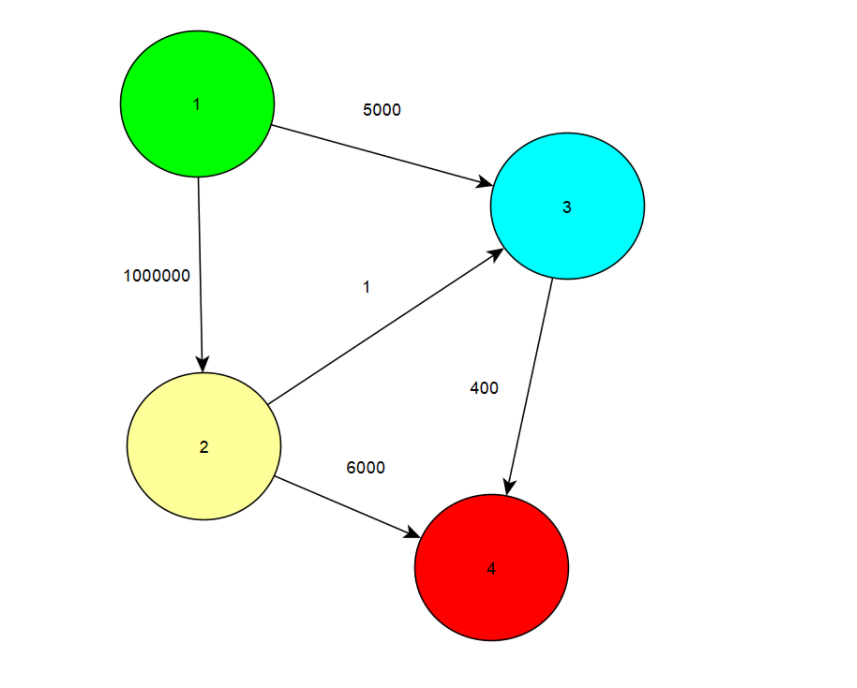
\includegraphics[height=15cm]{ex1.png}
	
	這是範例測資1、2的示意圖
\end{center}
\end{figure}

\ProblemSample{ex3.in}{ex3.out}

%\clearpage


\ProblemSubtaskTitle

本題共有 \total{ProblemSubtask} 組子任務,條件限制如下所示。

\begin{ProblemSubtaskTable}
    \ProblemSubtask{1}{題目範例}
    \ProblemSubtask{13}{$N,M,K \le 5$}
    \ProblemSubtask{27}{$K = 0$}
    \ProblemSubtask{21}{$K=1$}
    \ProblemSubtask{25}{$K \le 10$}
    \ProblemSubtask{13}{無額外限制}
\end{ProblemSubtaskTable}

\end{document}